
\documentclass{beamer}

\mode<presentation> {

    \usetheme{Madrid}
    \usecolortheme{beaver}
    %\setbeamertemplate{footline} % To remove the footer line in all slides uncomment this line
    %\setbeamertemplate{footline}[page number] % To replace the footer line in all slides with a simple slide count uncomment this line

    \setbeamertemplate{navigation symbols}{} % To remove the navigation symbols from the bottom of all slides uncomment this line
}
% \hypersetup{pdfpagemode=FullScreen}

\usepackage{multicol}
\usepackage{graphicx}
\usepackage{hyperref}
\usepackage{color}
\usepackage{booktabs} % Allows the use of \toprule, \midrule and \bottomrule in tables
\usepackage[T2A]{fontenc}
\usepackage[utf8]{inputenc}
\usepackage[english,russian]{babel}



%----------------------------------------------------------------------------------------
%   TITLE PAGE
%----------------------------------------------------------------------------------------

\title[Практика]{3D-Scanner with Kinect/LeapMotion}

\author{Васильев Роман}
\institute[СПбАУ]
{
Санкт-Петербургский \\
Национальный Исследовательский  \\
Академический Университет \\
Российской Академии Наук \\

\medskip{
Научный руководитель \\
% д. ф.-м. н., профессор\\
% Георгий Георгиевич Зегря
}
}
\date{\today}

\begin{document}

\begin{frame}
    \titlepage
\end{frame}

%----------------------------------------------------------------------------------------

\begin{frame}{Содержание}
    \tableofcontents 
\end{frame}

%----------------------------------------------------------------------------------------
%   PRESENTATION SLIDES
%----------------------------------------------------------------------------------------


\section{Введение}

\begin{frame}{Введение}
    \begin{itemize}
        \item Цель
        \begin{itemize}
            \item Разработать 3D-сканер
        \end{itemize}
        \item Задачи
        \begin{itemize}
            \item Изучить API RGB-D сенсоров
            \item Разработка аппаратной части сканера
            \item Разработка алгоритма построения 3D-модели
        \end{itemize}
        \item Результат
        \begin{itemize}
            \item Разработать 3D-сканер
        \end{itemize}
    \end{itemize}
    
\end{frame}


% \section{Мотивация}

% \begin{frame}{Мотивация}
    
% \end{frame}


\section{Что использовалось?}

\begin{frame}{Что использовалось?}
    \begin{itemize}
        \item Для получение данных с Kinect использовалась библиотека libfreenect, написанная на C. Работа с кинектом происходила при помощи интерфейсов, написанных на C++.
        \item Для обработки облаков точек использовалась библиотека Point Cloud Library. Из-за того, что шаблонные классы каждый раз долго пересобирались, была собрана динамическая библиотека с нужными интерфейсами.
        \item Все интерфейсы были обернуты в классы Python при помощи SWIG для удобства работы.
        \item Чуть-чуть кода для Arduino на C.
    \end{itemize}

    Весь код находится в репозитории \href{https://github.com/nizshee/scannect}{\color{blue}https://github.com/nizshee/scannect}
\end{frame}


\section{Оборудование}

\begin{frame}{Kinect}
    \begin{columns}[T]
        \begin{column}[T]{5cm}
            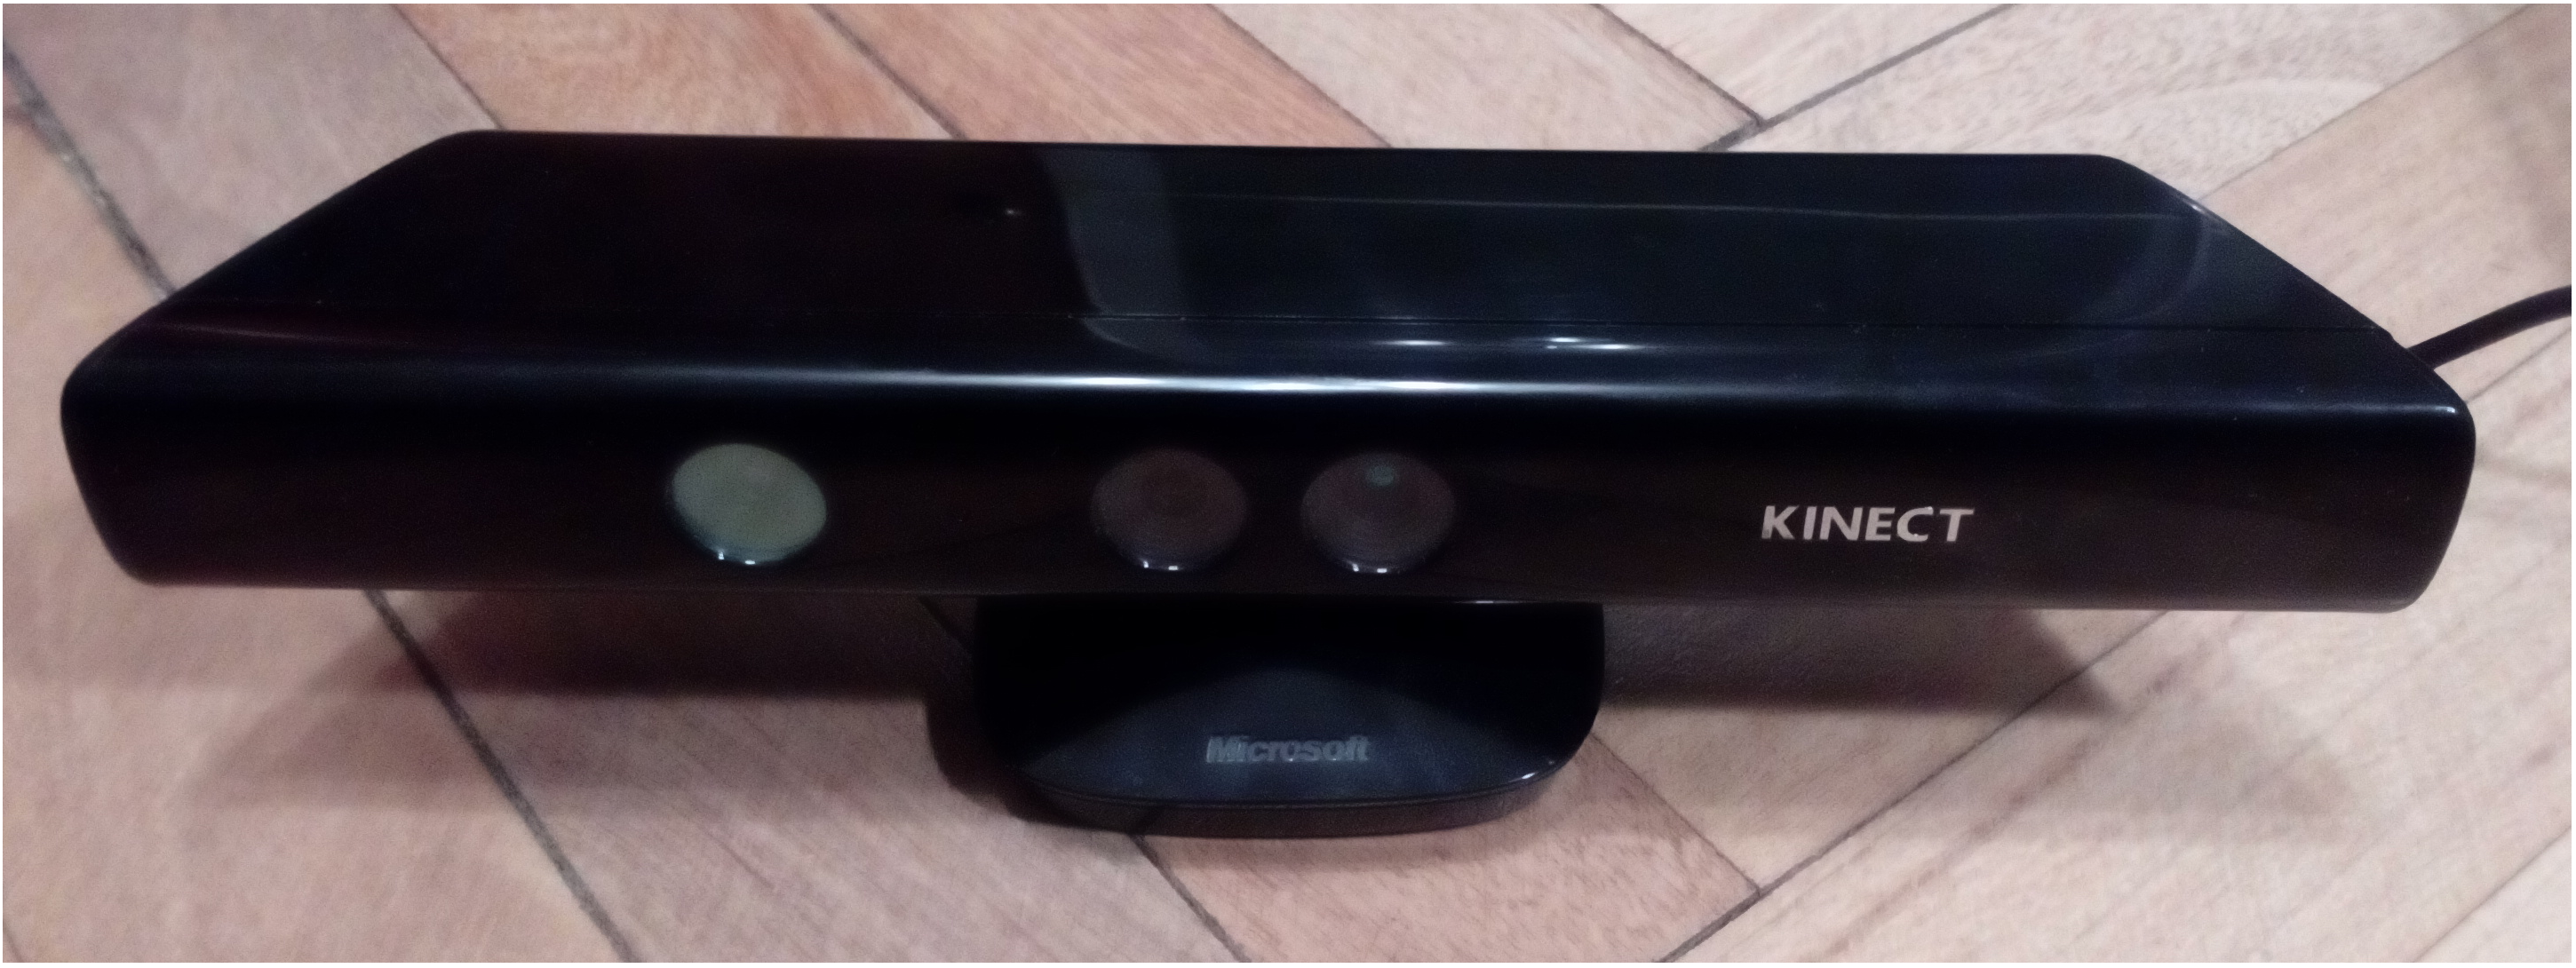
\includegraphics[scale=0.045]{kinect1}\\
            Kinect — бесконтактный сенсорный игровой контроллер, первоначально представленный для консоли Xbox 360, и значительно позднее для персональных компьютеров.
            Предполагается, что компьютер работает под управлением Windows.
        \end{column}

        \begin{column}[T]{5cm}
            Состав:
            \begin{itemize}
            \item Color Sensor - просто камера
            \item IR Emitter - инфракрасный излучатель
            \item IR Depth Sensor - инфракрасный приемник. 
            \end{itemize}
            Максимальное разрешение карты глубины 640x480 (30 fps). 
        \end{column}
    \end{columns}
    \begin{center}
    \small

    \end{center}

\end{frame}

\begin{frame}{Крутящаяся подставка}
    \begin{columns}[T]
        \begin{column}[T]{5cm}
            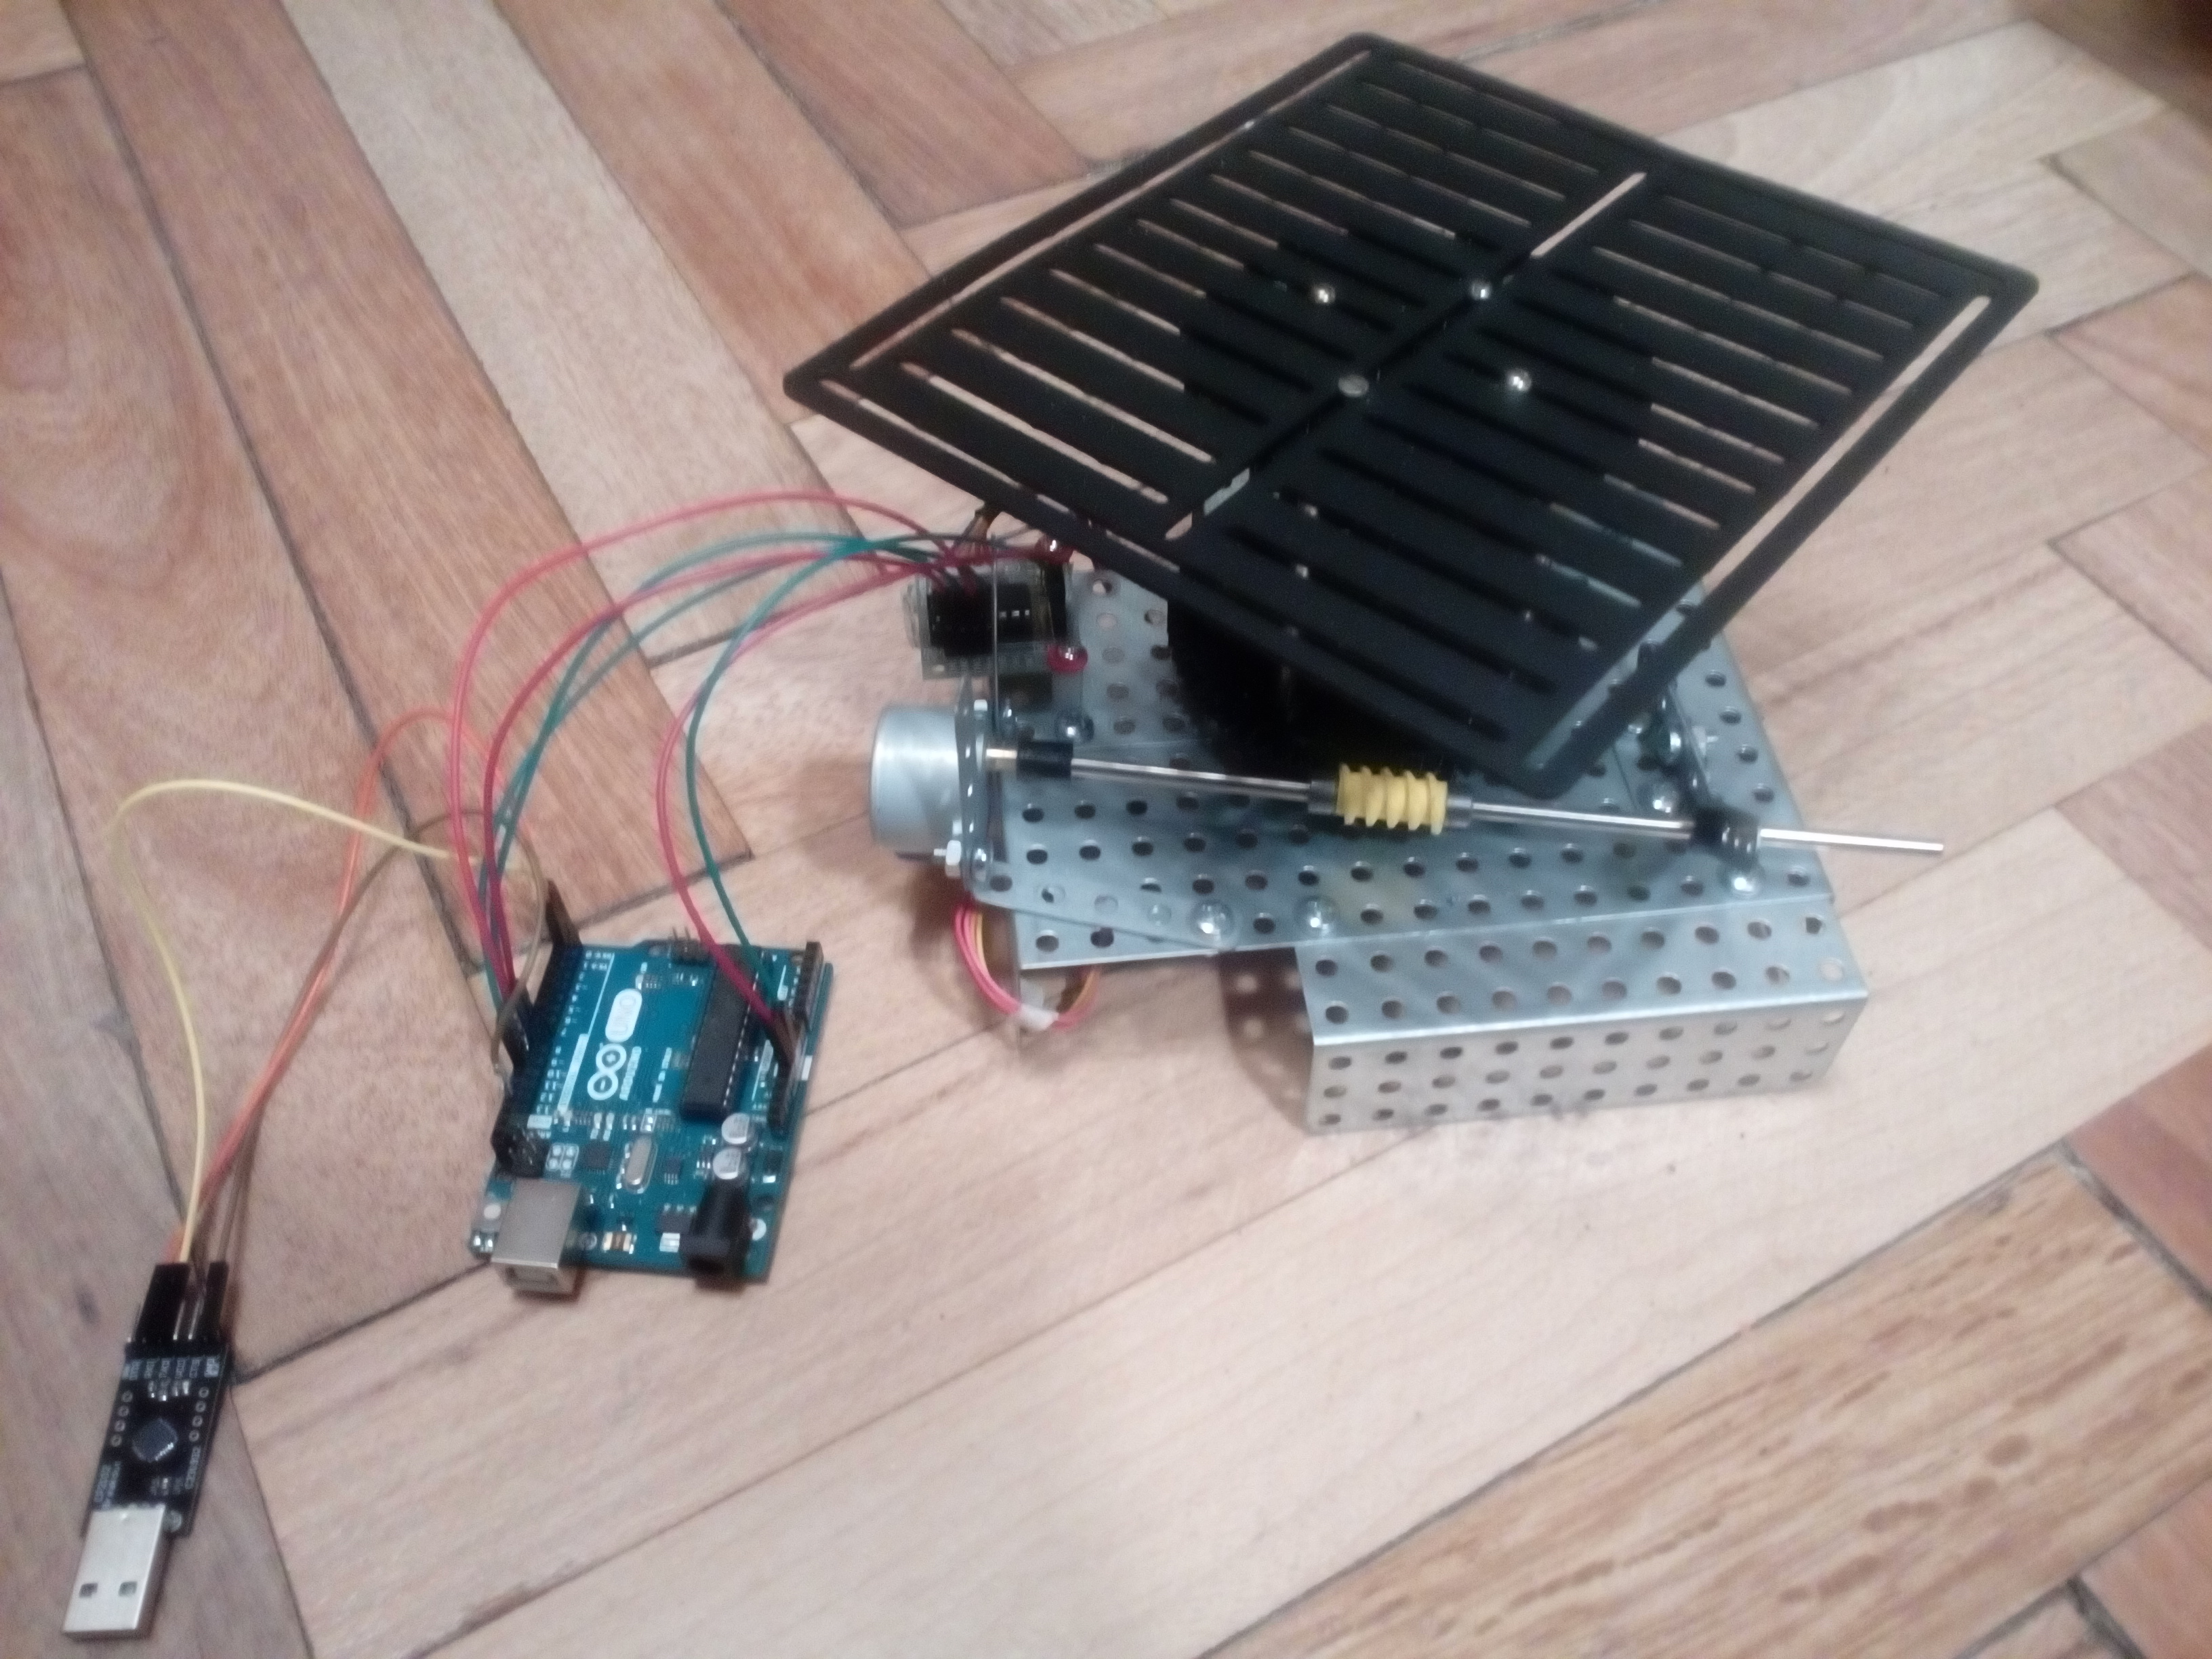
\includegraphics[scale=0.04]{device}\\
            \small
            Состоит из:
            шагового двигателя (поворот подставки),
            Arduino (прием комманд и управление шаговым двигателем) 
            и безымянного конструктора.
        \end{column}
        \begin{column}[T]{5cm}
            С помощью библиотеки PySerial через цифровые порты ввода/вывода (RX/TX) подаются команды на Arduino, на какой угол нужно развернуть подставку.
            \vspace*{2\baselineskip}

            Поворот с точностью $\sim 1$ градуса.
        \end{column}
    \end{columns}
\end{frame}


\begin{frame}{Установка}
    \begin{columns}[T]
        \begin{column}[T]{5cm}
            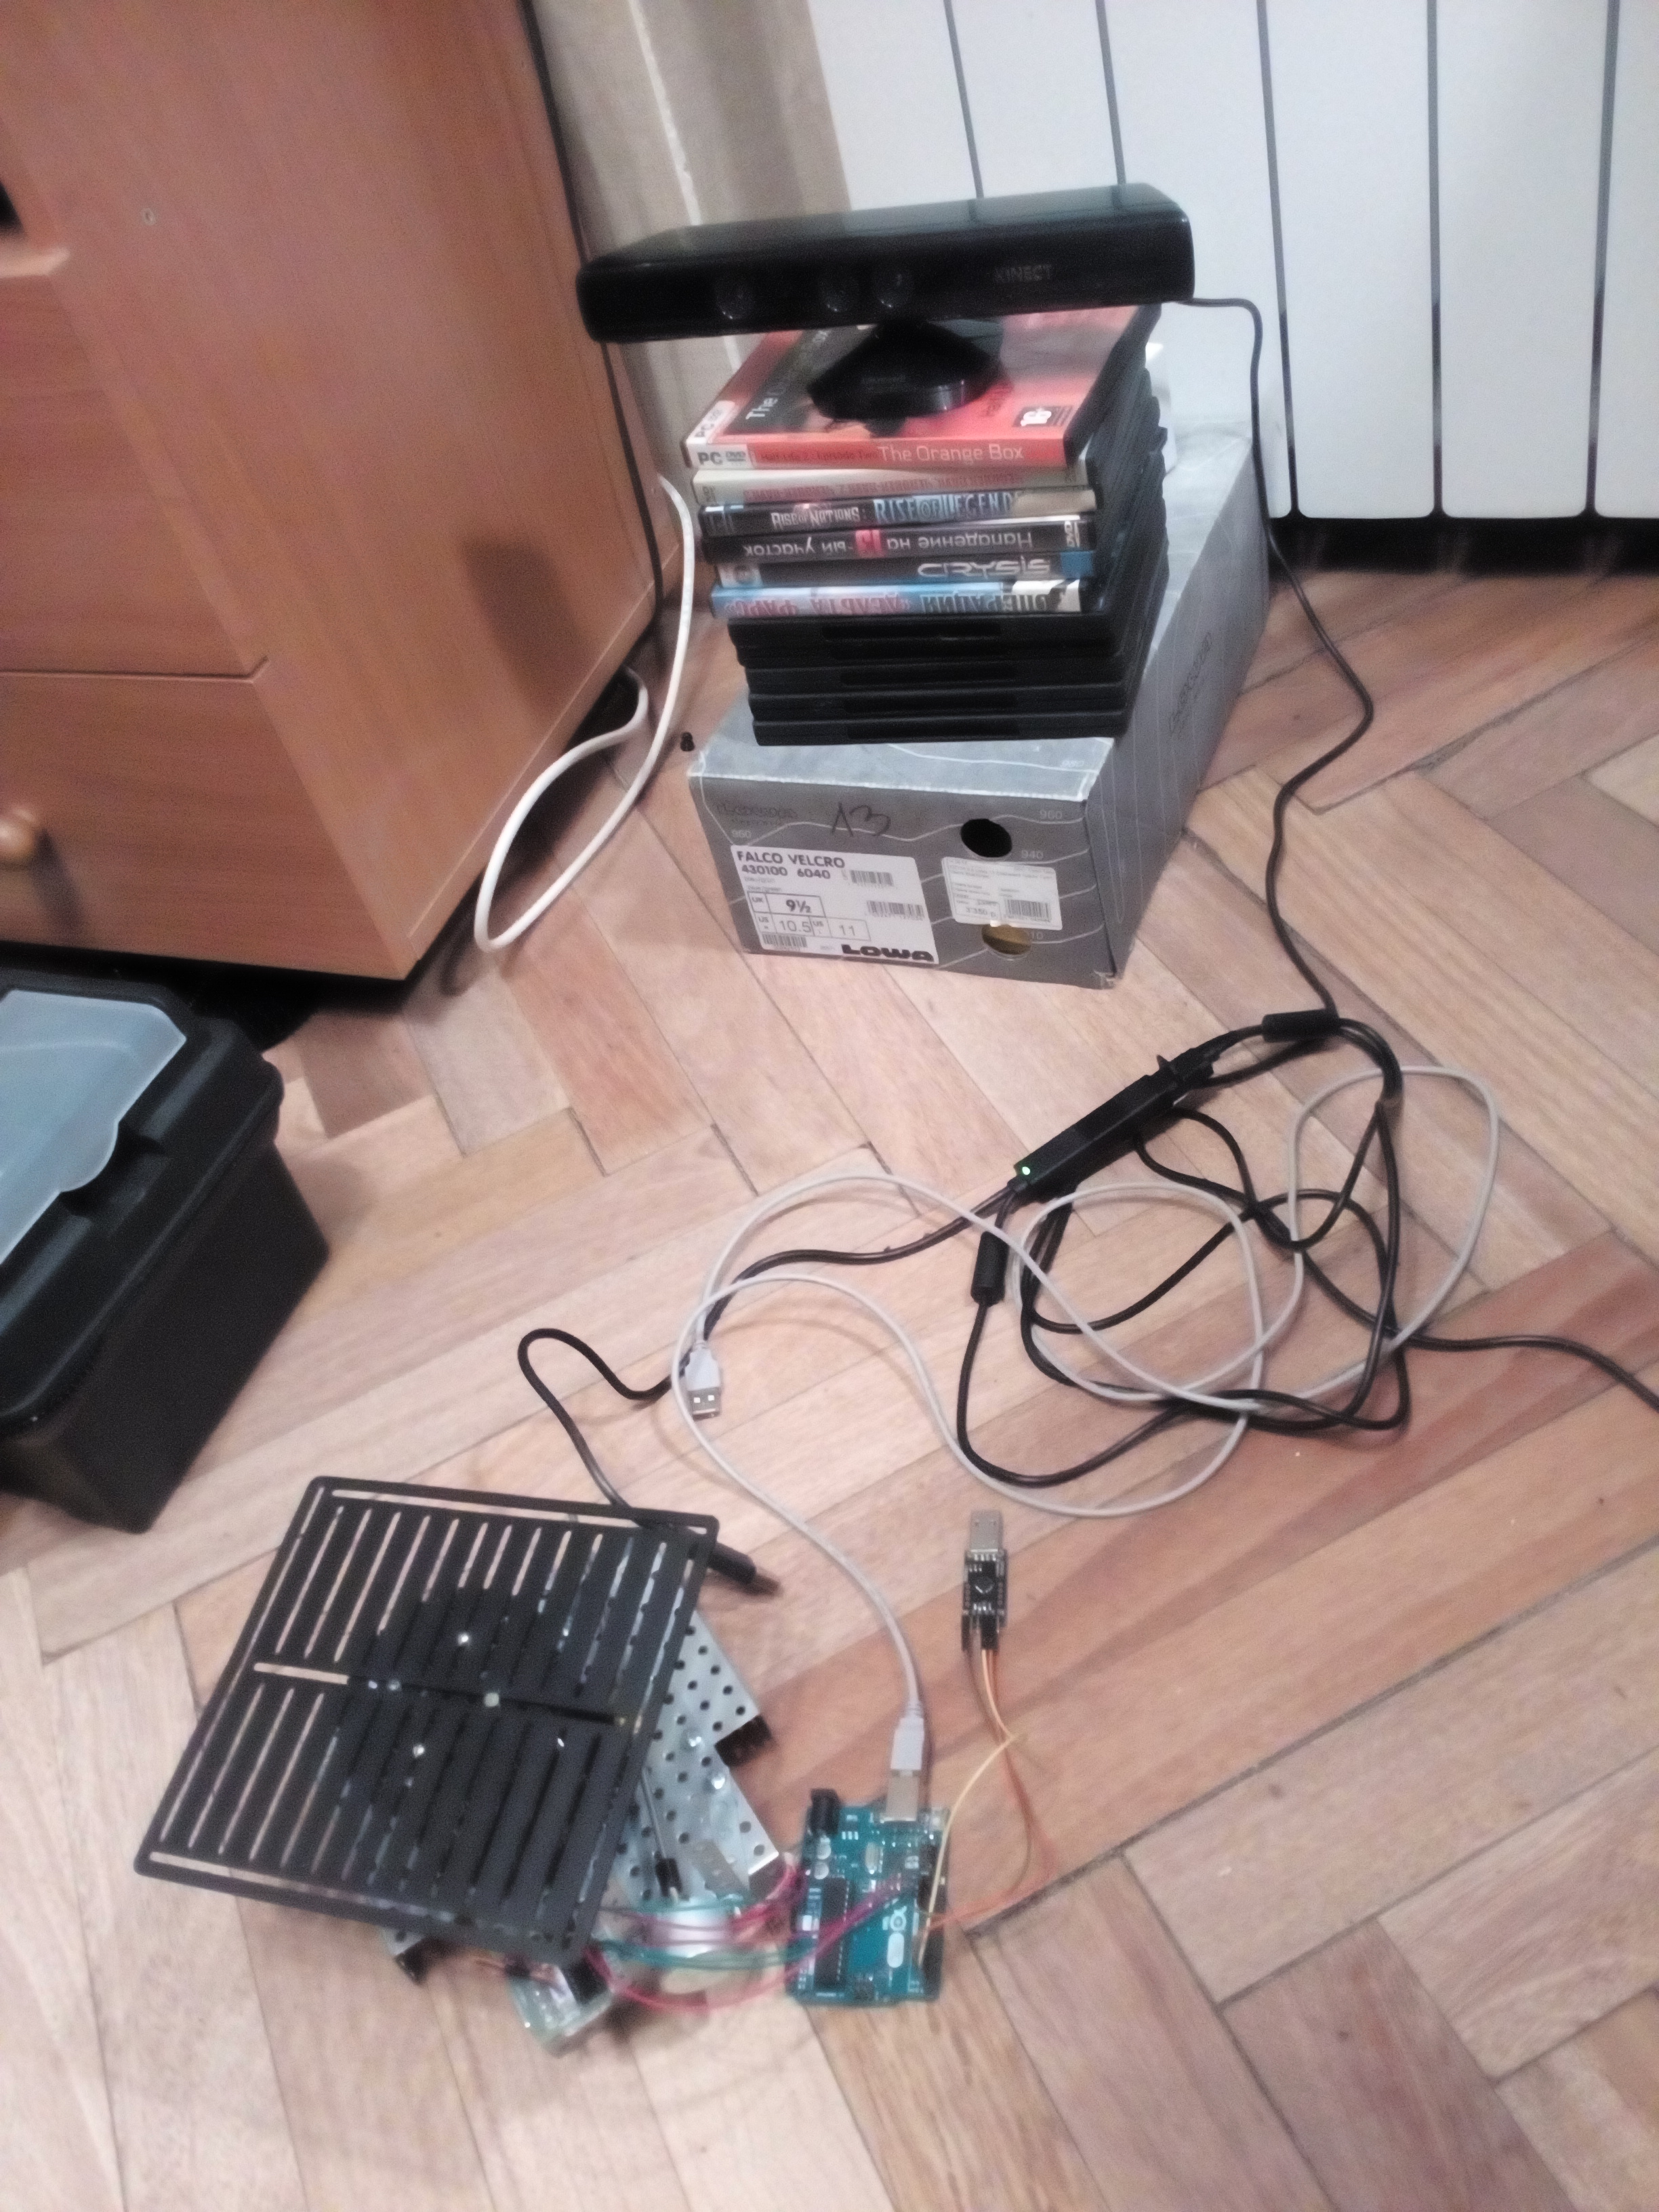
\includegraphics[scale=0.06]{devices}
        \end{column}
        \begin{column}[T]{5cm}
            \small
            Kinect поднят для того, чтобы  был виден верх образца. \\
            Принцип работы:
            \begin{itemize}
            \item
            Образец сканируется при помощи Kinect, поворачивается на небольшой угол, снова сканируется и т.д.
            \item
            После этого полученные облака точек накладываются друг на друга (при помощи ndt) и сливаются в одно большое скопление точек.
            \item
            Оно сглаживается и фильтруется.
            \end{itemize}

        \end{column}
    \end{columns}
\end{frame}


\section{Пример}

\begin{frame}{Пример}
    \begin{columns}[T]
        \begin{column}[T]{7cm}
            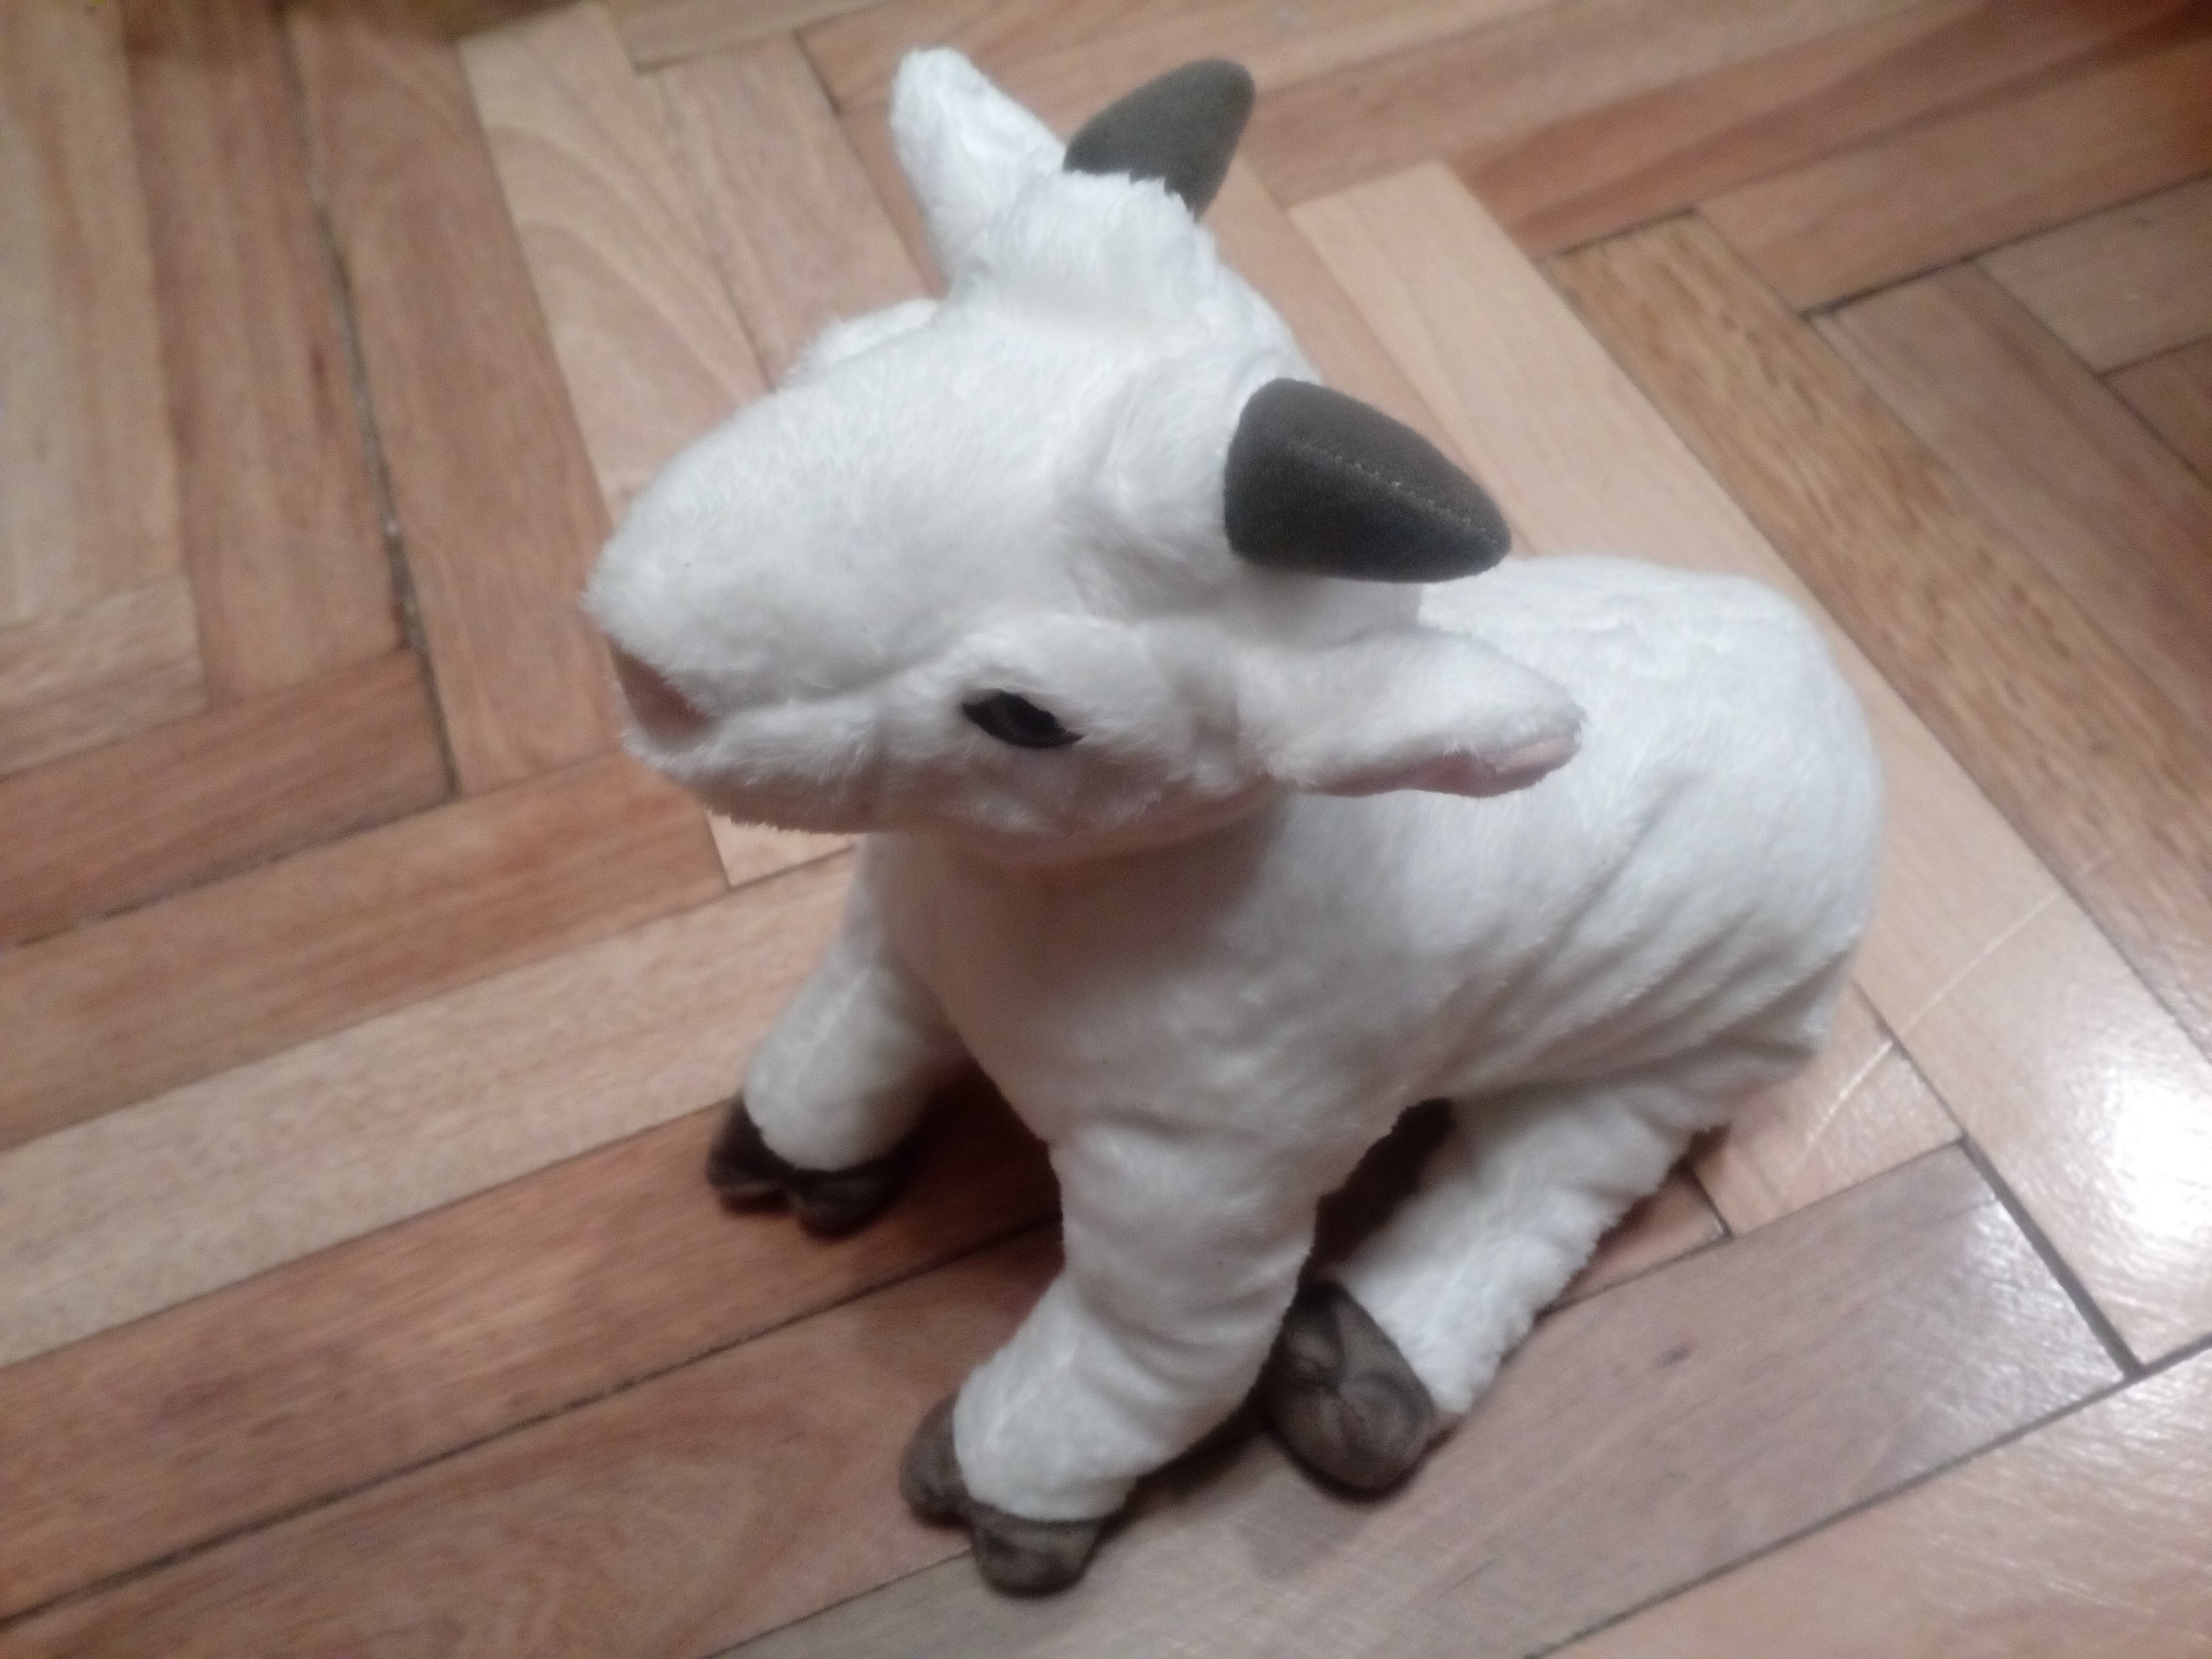
\includegraphics[scale=0.06]{sheep}\\
        \end{column}
        \begin{column}[T]{5cm}
            Попытка оцифровать козлика.

            Стоит учесть, что козлик был достаточно большим и имел сложную форму. 

            Поэтому некоторые участки содержат больше точек, некоторые меньше.
        \end{column}
    \end{columns}
\end{frame}


\begin{frame}{Пример}
    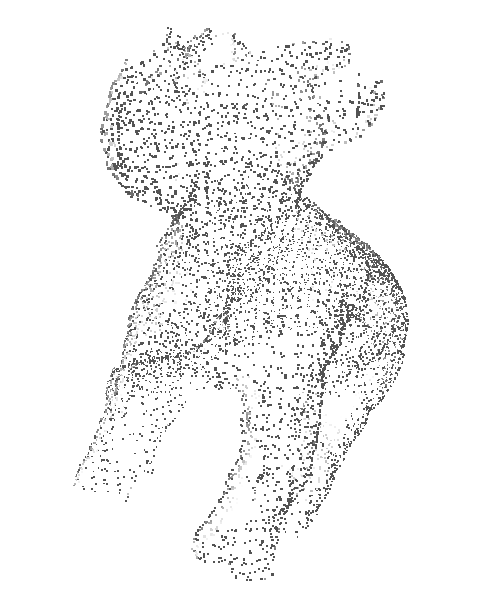
\includegraphics[scale=0.45]{snapshot02a}
    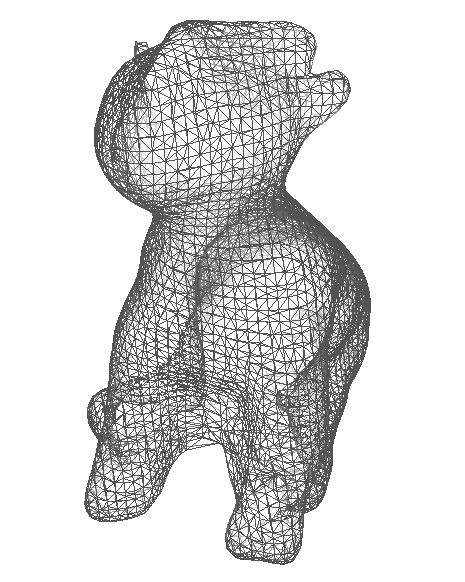
\includegraphics[scale=0.45]{snapshot04a}
\end{frame}


\section{Итог}

\begin{frame}{Итог}
    \begin{center}
        \begin{itemize}
        \item
        Получилось сделать прототип 3D-сканера.
        \item
        Можно делать 3D-модели объектов, которые не сильно изменяются при поворотах (но при этом изменяются).
        \item
        Хуже дела обстоят с объектами, типа параллелепипедов.
        \item
        Можно было бы добавить окраску точек в соответсвуюцие цвета.
        \end{itemize}
    \end{center}
\end{frame}

\begin{frame}
\Huge{\centerline{Спасибо!}}
\end{frame}

%----------------------------------------------------------------------------------------

\end{document}